\subsection{Constrained nonlinear transfer}
Four objects were fixed by geometry and material representation before validation. At $k=8$, both policies use the same initialization, prior, damping schedule, material constraints and full-objective Armijo line search. Only the tangent-current policy changes. Three paired trajectories complete all 18 updates. Table~\ref{tab:nonlinear} reports their complete-volume material errors and held-out data errors.

\begin{table*}[t]\centering
\caption{Constrained nonlinear transfer: receiver $\rightarrow$ verified exchange. Material errors are relative full-volume norms. Child wall includes each policy's own physical setup, acquisition, all outer work and terminal evaluation. Each trajectory is timed once.}\label{tab:nonlinear}
\begin{tabular}{lrrrr}\toprule
Geometry / material tangent&Complex material&Real material&Imaginary material&Held-out data\\\midrule
Smooth / voxel&$0.3027\to0.2699$&$0.2811\to0.2516$&$0.7439\to0.6506$&$0.006637\to0.002836$\\
Near-contact / Gaussian&$0.6722\to0.6707$&$0.6810\to0.6835$&$0.4439\to0.2859$&$0.010521\to0.007080$\\
Shell / Gaussian&$0.6096\to0.5660$&$0.6081\to0.5651$&$0.6976\to0.6219$&$0.014190\to0.012179$\\\midrule
Geometry / material tangent&\multicolumn{2}{c}{Child wall (s)}&Wall ratio&Total full tangent RHS\\
Smooth / voxel&\multicolumn{2}{c}{$216.5\to579.9$}&2.68&$0\to708$\\
Near-contact / Gaussian&\multicolumn{2}{c}{$407.7\to710.5$}&1.74&$0\to744$\\
Shell / Gaussian&\multicolumn{2}{c}{$405.9\to592.3$}&1.46&$0\to744$\\\bottomrule
\end{tabular}
\end{table*}

Complex-material error decreases by 10.8\%, 0.22\%, and 7.16\%, respectively, and held-out errors decrease in all three pairs. The near-contact real-part error increases slightly, so improved data fit does not imply uniform component recovery. The fourth object's exchange trajectory retains 17 completed updates. Before update 18, its receiver-derived starting endpoint fails the fixed normal-residual check, stopping that exchange trajectory. The separate receiver-only baseline job is not run after the queue stops. The four-object denominator and both unavailable final endpoints remain explicit.

These trajectories support a limited reconstruction consequence of the frozen rule. They also separate fidelity from efficiency: the complete child-wall ratios range from 1.46 to 2.68. Extra tangent actions purchase checked material changes; faster imaging is not established.

\begin{figure*}[t]\centering
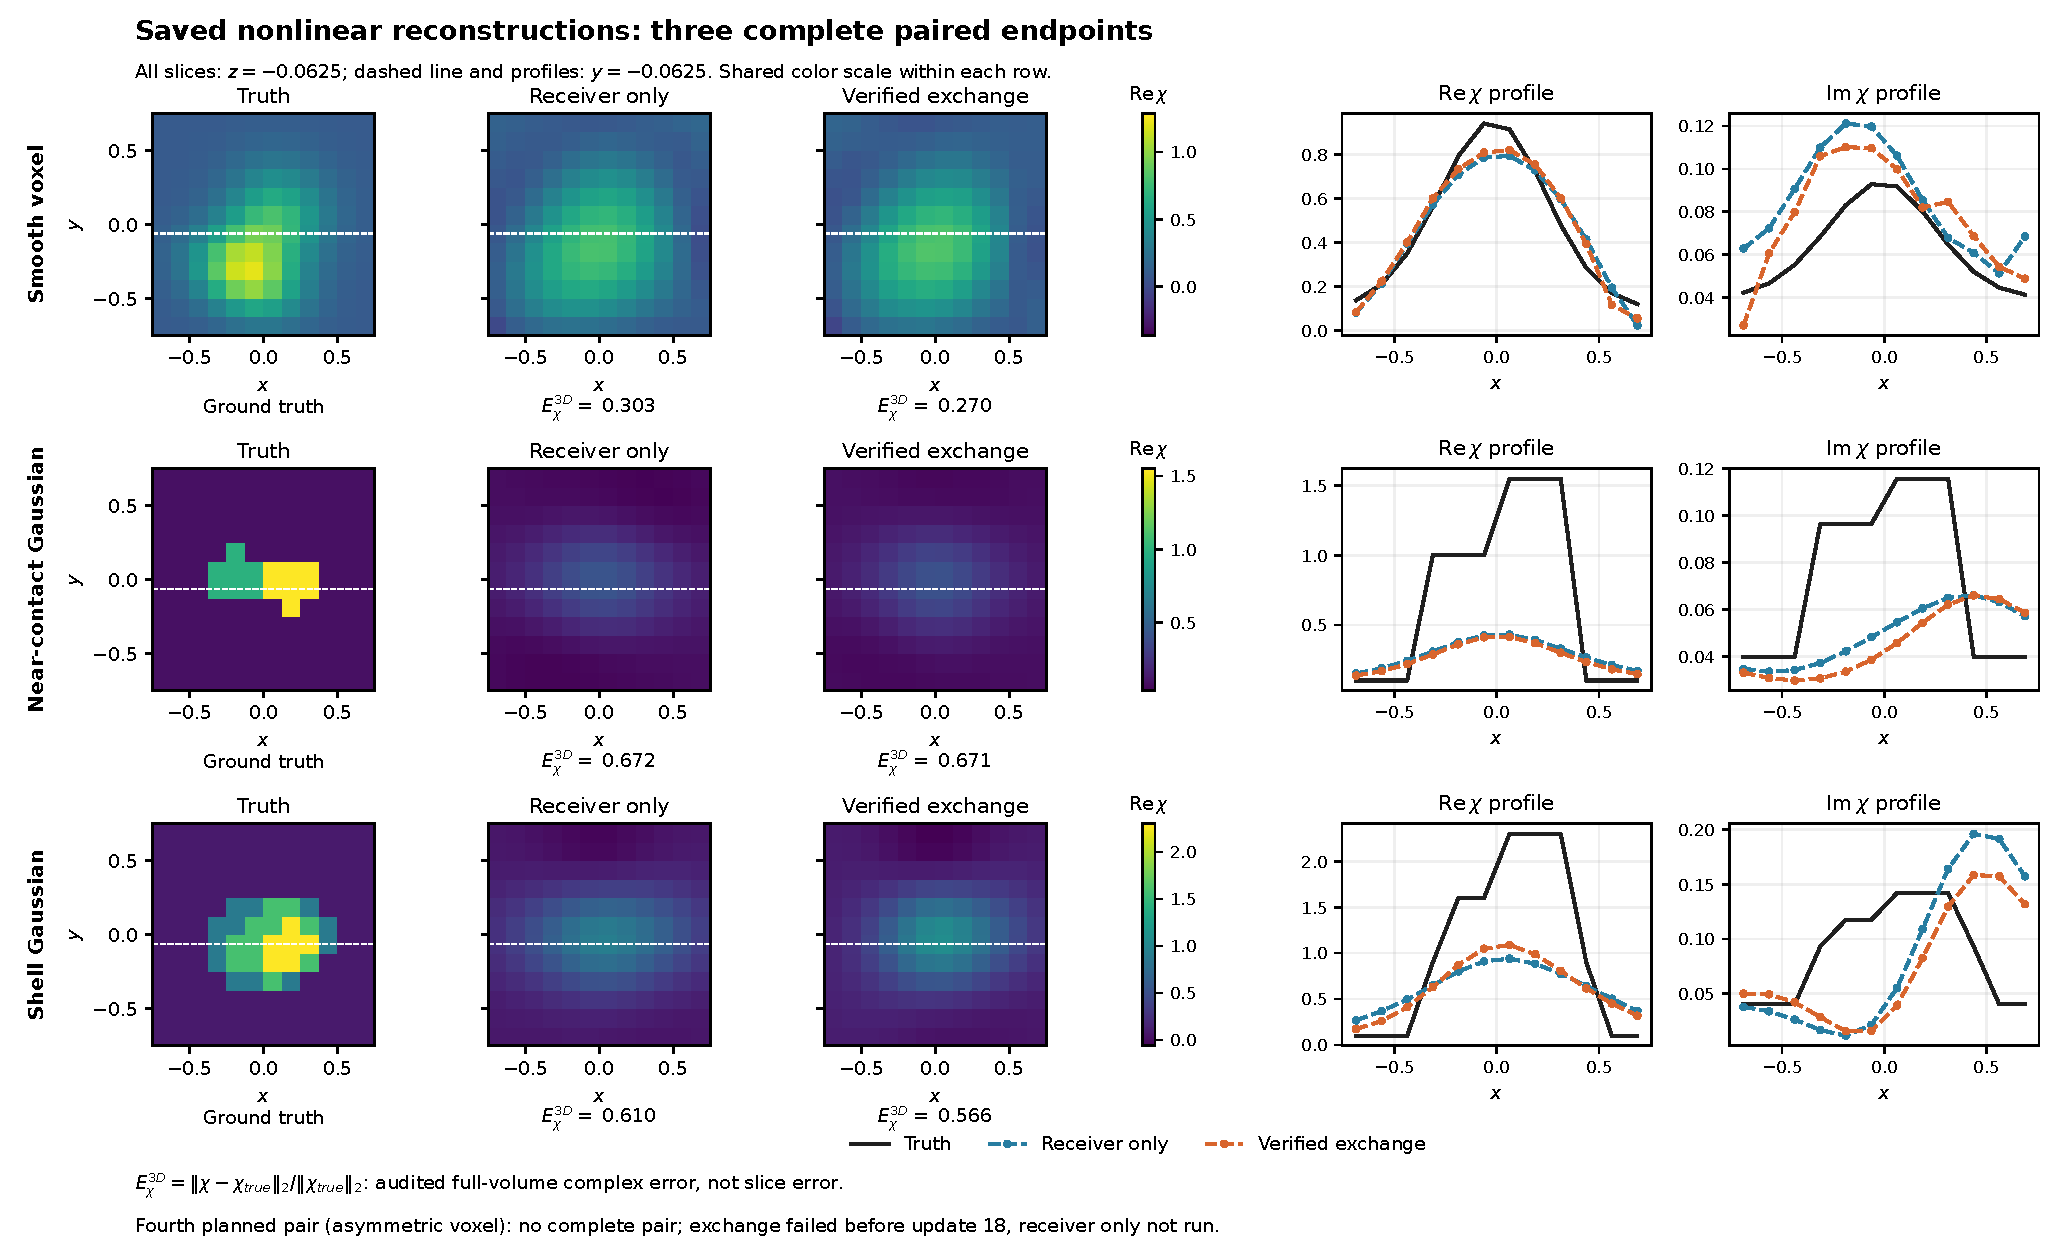
\includegraphics[width=.92\textwidth]{figures/nonlinear_closure_v1/nonlinear_reconstructions.pdf}
\caption{Complete nonlinear pairs at current rank eight. The real-material slices use the same central inverse-grid plane and a common color scale within each row; line profiles compare both real and imaginary contrast. These images accompany complete-volume errors in Table~\ref{tab:nonlinear}. The contact and shell peaks remain blurred despite improved data fit. The asymmetric voxel pair has no completed paired endpoint and is retained separately in the failure record.}\label{fig:nonlinear-slices}
\end{figure*}
